\documentclass[crop=false,a4paper,oneside,11pt]{standalone}
\usepackage{a4wide,graphicx,fancyhdr,amsmath,amssymb,float,graphicx,color,geometry,xcolor,titlesec,colortbl,tabu}
\usepackage[parfill]{parskip}
\usepackage[nodayofweek]{datetime}
%----------------------- Macros and Definitions --------------------------

%fast change of things
\newcommand{\mysubject}{2IO70 DBL Embedded Systems}
\newcommand{\myassignment}{Group 12}

%\definecolor{titlepagecolor}{cmyk}{1,.60,0,.40}
%\definecolor{namecolor}{cmyk}{1,.50,0,.10}


\setlength\headheight{20pt}
\addtolength\topmargin{-10pt}
\addtolength\footskip{20pt}

% Define light and dark Microsoft blue colours
\definecolor{MSBlue}{rgb}{.204,.353,.541}
\definecolor{MSLightBlue}{rgb}{.31,.506,.741}
\arrayrulecolor{MSLightBlue}

% Set formats for each heading level

\titleformat*{\section}{\Large\bfseries\sffamily\color{MSBlue}}
\titleformat*{\subsection}{\large\bfseries\sffamily\color{MSLightBlue}}

%date format
\newdateformat{mydate}{\monthname[\THEMONTH] \THEYEAR}

\fancypagestyle{plain}{%
\fancyhf{}
\renewcommand{\headrulewidth}{0pt}
\renewcommand{\footrulewidth}{0pt}
}

\pagestyle{fancy}
\fancyhf{}
\fancyfoot[CO] {\thepage}
\renewcommand{\headrulewidth}{0pt}
\renewcommand{\footrulewidth}{0pt}


%--------------------------------- Text ----------------------------------
\setcounter{secnumdepth}{0}
\begin{document}

\section{Experimental Evaluation}

We ran all the tests in our experimental evaluation on a HP EliteBook 8570w with an Intel i7-3630QM CPU @ 2.40GHz and 8,00 GB RAM. To measure the amount of time and algorithm we start a timer in the code just before the part we want to test and we stop the timer right after the part stops. For testing the 2-position, 4-position and 1-slider algorithms we generated test cases with $5$ different distributions. These distributions are:
\begin{enumerate}
    \item Uniform. Points are randomly placed on a $10000$ by $10000$ plane.
    \item Clustered. Points are placed around $20$ randomly chosen points.
    \item H Clustered. Points are placed around $10$ randomly chosen $y$-coordinates.
    \item V Clustered. Points are placed around $10$ randomly chosen $x$-coordinates.
    \item Bounded. Points are randomly placed on a $1000$ by $1000$ plane.
\end{enumerate}
We have $500$ test cases in total, $100$ of each different distribution with $5$ different label sizes. The label sizes are, $100$ by $100$, $100$ by $500$, $500$ by $100$, $1000$ by $1000$ and $5000$ by $5000$.

\subsection{2-position}
\subsubsection{Results}
The algorithm of 2-position model has been explained in the previous section. As a recap this algorithm has two phase: first we map all the collisions of every candidates of every single point, then we try to place the candidates that has least amount of collisions. Since it give a clear expression of mapping collisions and placing labels with least collisions. In theory, it is most likely to find a optimal solution. For this experimental evaluations we use $2500$ different test cases with $500$ cases for each distributions. The following picture shows an example of the labels placement in one of the cases(Red point mean there are no labels can be placed). As you can see, the solution we found is quite optimal in this area.

\begin{figure}[h!]
\centering
  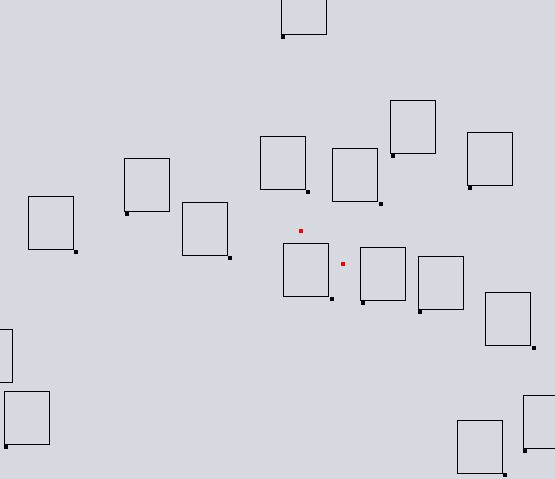
\includegraphics[scale = 0.5]{2pos_example.JPG}\\
  \caption{A graphic showing an example of the 2-position algorithm}
 \end{figure}

The running time of the 2-position algorithm can be seen in the following figure. This graph shows the running time of five different distributions which has amount of points from $100$ to $10000$ with $100$ in between.
\begin{figure}[h!]
 \centering
  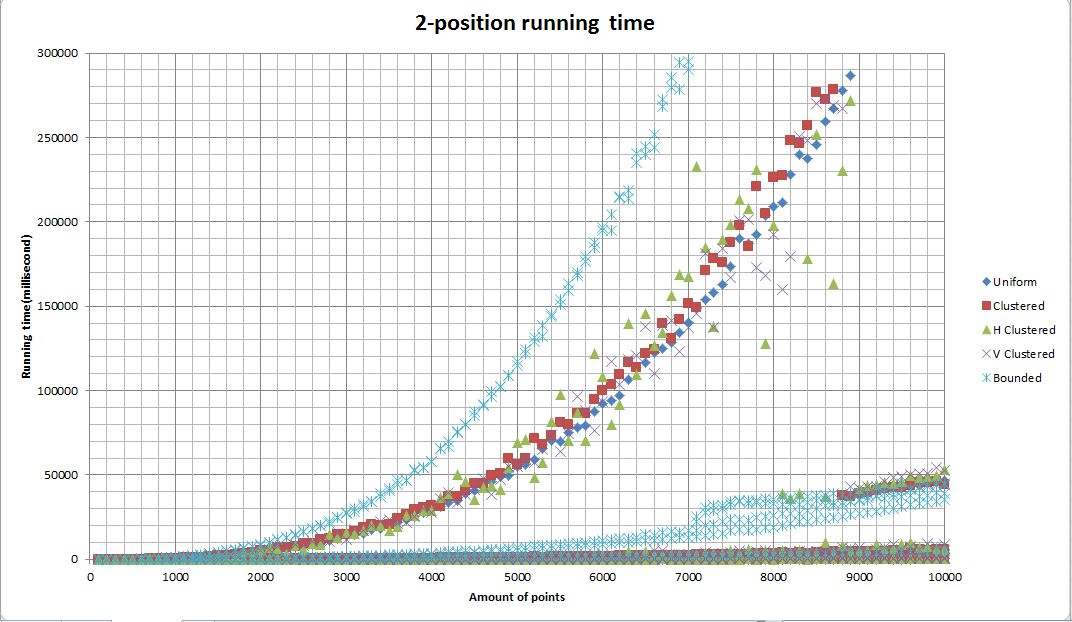
\includegraphics[scale = 0.5]{2PosRunningTime.JPG}\\
  \caption{A graphic showing the percentage of labels placed by the 4-position algorithm}
 \end{figure}

The following graph shows the percentage of label placed by 2-position algorithm. It also shows five different types of distribution.
\begin{figure}[h!]
 \centering
  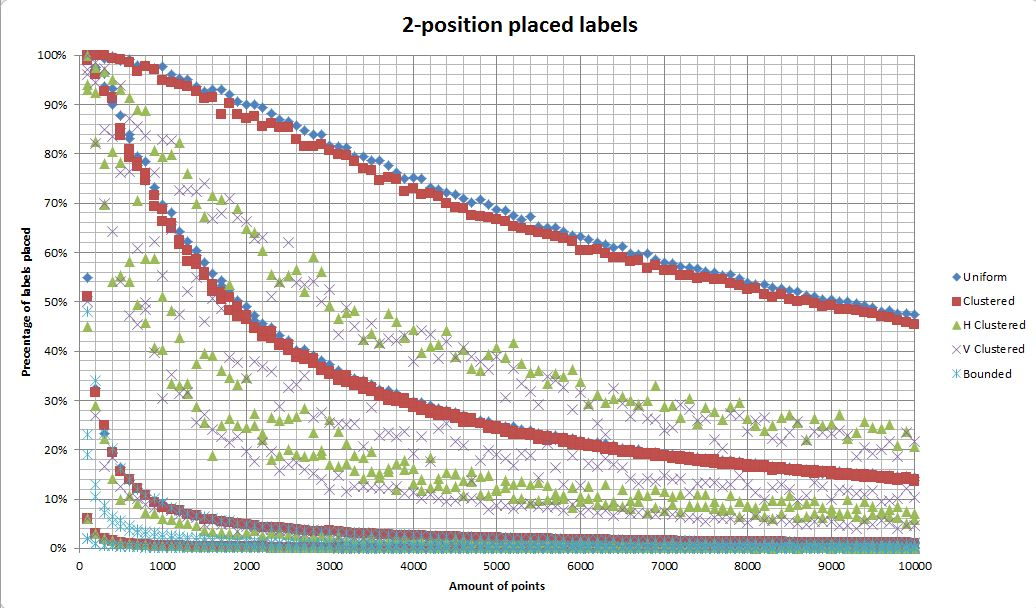
\includegraphics[scale = 0.5]{2PosLabelsPlaced.JPG}\\
  \caption{A graphic showing the percentage of labels placed by the 4-position algorithm}
 \end{figure}
\subsubsection{Discussion}
As we explained in the previous section. The theoretical running time of the whole 2-position algorithm will take $O(n^2)$. In figure $2$, it shows the running time of $2500$ different cases. You can see most of the cases are quite low in the running time and also close to their best cases. That's because the amount of collisions of the candidates are very small, so it won't take much time to map the collisions and it take less time to place the labels. There are some cases that have higher running time than the others. And we can see from the figure that the practical worst case running time are close to the theoretical running time $O(n^2)$ as we explained before. \\
You can also find out the worst cases of each distribution suddenly drops when the number of points reaches a specific amount. That's because in these cases, there are too many collisions. If we use the regular algorithm, the running time will become really high so it's not efficient. So in that case, we use greedy algorithm to place the labels. The running time will become lower and the solution is as optimal when using the regular algorithm since there are a lot of collisions.\\
Other than running time, we also look at the results of our algorithm. As we can see from figure $3$, when the amount of points are small, the algorithm gives nice solutions with high percentage of placed labels. When the amount of points become higher, the percentage of placed labels will become lower. This is pretty normal since the labels have the same height and the same width for the same type of distribution but with different amount of points. Even in the cases with $10000$ points, we still have more than $50\%$ label placement. The reason why bounded cases have low solution is because all points are collapsed in a small area.\\
As this algorithm is considered very efficient and gives optimal results in different distributions, we consider this algorithm as the optimal solution for this problem.

\subsection{4-position}
\subsubsection{Results}
The running time of the 4-position algorithm can be seen in figure ...
 \begin{figure}[h!]
 \centering
 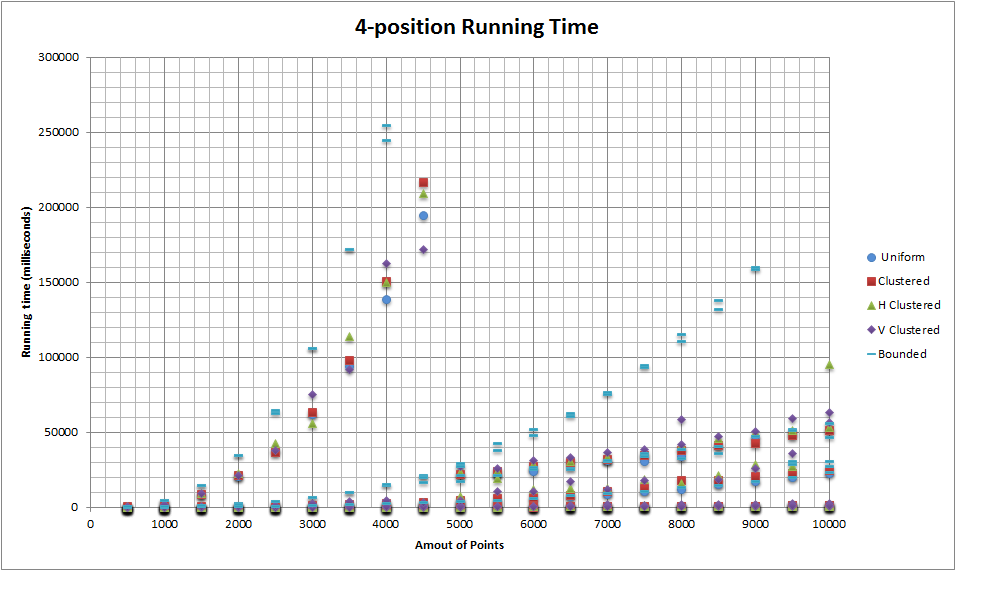
\includegraphics[scale = 0.5]{4PosRunningTime.png}\\
 \caption{A graphic showing the Running Time of the 4-position algorithm}
 \end{figure}

The percentage of labels placed by the 4-position algorithm can be seen in figure ...
 \begin{figure}[h!]
 \centering
  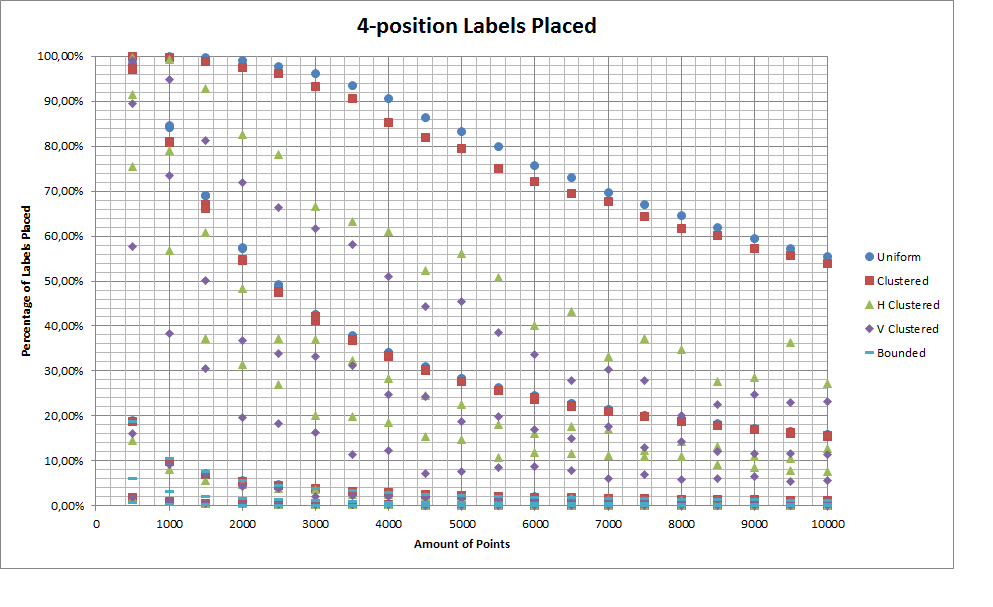
\includegraphics[scale = 0.5]{4PosLabelsPlaced.png}\\
  \caption{A graphic showing the percentage of labels placed by the 4-position algorithm}
 \end{figure}
\subsubsection{Discussion}

\subsection{1-slider}
\subsubsection{Results}
The running time of the 1-slider algorithm can be seen in figure ... We found in practice that the running time of the 1-slider algorithm can exceed the time limit we had of 5 minutes when the amount of overlaps was large. We thus put a hard limit of 4.5 minutes on the heuristic algorithm and, if the algorithm had not given a result by then, ran a greedy algorithm.

The percentage of labels placed by the 1-slider algorithm can be seen in figure ...
\subsubsection{Discussion}

\end{document}
